Das $v(t)$-Diagramm (oben) beschreibt die Bewegung eines Körpers auf einer geraden Linie; bei $t = 0$ ist er bei $s = 0$. Ein Schüler hat dazu das $s(t)$-Diagramm (unten) skizziert, in vier Stücken. Eines davon ist falsch.
\begin{center}
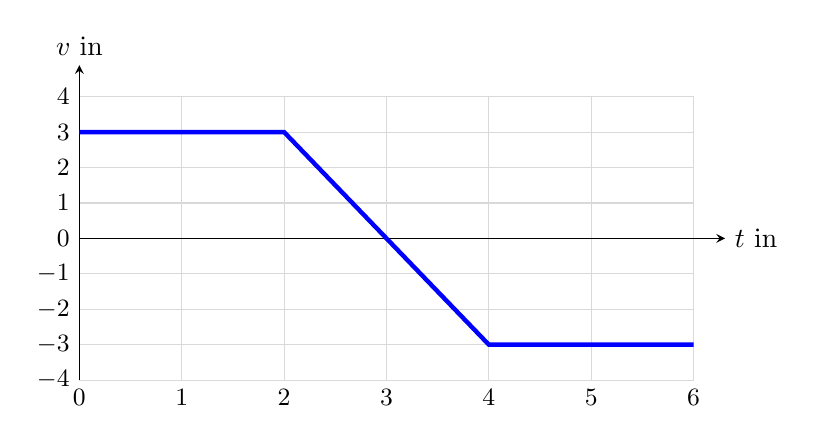
\begin{tikzpicture}[>=stealth, x=1.3cm, y=0.45cm]
 \draw[gray!30] (0,-4) grid[xstep=1, ystep=1] (6,4);
 \draw[->] (0,0) -- (6.308,0) node[right] {$t$ in \si{\second}};
 \draw[->] (0,-4) -- (0,4.889) node[above] {$v$ in \si{\meter\per\second}};
 \foreach \tk in {0,1,2,3,4,5,6} \node[below] at (\tk,-4) {\small $\tk$};
 \foreach \yk in {-4,-3,-2,-1,0,1,2,3,4} \node[left] at (0,\yk) {\small $\yk$};
 \draw[ultra thick, blue] (0,3) -- (2,3) -- (4,-3) -- (6,-3);
\end{tikzpicture}
\end{center}\begin{center}
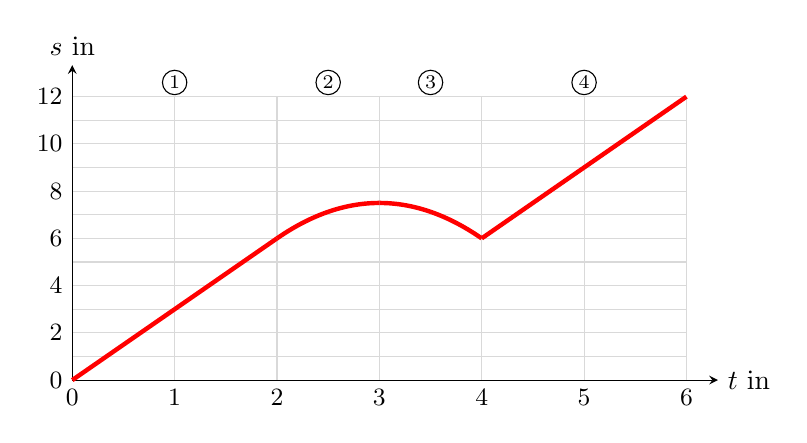
\begin{tikzpicture}[>=stealth, x=1.3cm, y=0.3cm]
 \draw[gray!30] (0,0) grid[xstep=1, ystep=1] (6,12);
 \draw[->] (0,0) -- (6.308,0) node[right] {$t$ in \si{\second}};
 \draw[->] (0,0) -- (0,13.333) node[above] {$s$ in \si{\meter}};
 \foreach \tk in {0,1,2,3,4,5,6} \node[below] at (\tk,0) {\small $\tk$};
 \foreach \yk in {0,2,4,6,8,10,12} \node[left] at (0,\yk) {\small $\yk$};
 \draw[ultra thick, red] (0,0) -- (2,6);
 \draw[ultra thick, red, domain=2:3, samples=30] plot (\x, {6+3*(\x-2)-1.5*(\x-2)*(\x-2)});
 \draw[ultra thick, red, domain=3:4, samples=30] plot (\x, {7.5-1.5*(\x-3)*(\x-3)});
 \draw[ultra thick, red] (4,6) -- (6,12);
 \node[circle, draw, inner sep=1pt, font=\scriptsize, fill=white] at (1,12.6) {1};
 \node[circle, draw, inner sep=1pt, font=\scriptsize, fill=white] at (2.5,12.6) {2};
 \node[circle, draw, inner sep=1pt, font=\scriptsize, fill=white] at (3.5,12.6) {3};
 \node[circle, draw, inner sep=1pt, font=\scriptsize, fill=white] at (5,12.6) {4};
\end{tikzpicture}
\end{center}
\begin{abcliste}
\abc Welches Stück ist falsch?
\abc Welchen Fehler hat der Schüler gemacht? Wo ist der Körper bei \tEO\ wirklich?
\end{abcliste}
